\section{Classes}
\label{sec:classdiagrams-classes}

This section describes the main properties of classes. 
These properties are shown and can be edited in the \code{Overview} tab of the properties view which is shown when a class is selected on the class diagram canvas.
The other properties tabs of the class relate to relationships between classes or children of classes and are described in later sections.

Classes represent sets of elements. 
The set can be a given type (\code{Carrier Set}), a constant subset (\code{Constant}) or a variable subset (\code{Variable}).
The kind of the class is decided by linking it to an existing data element in the Event-B model.
This link is called \code{elaborates} and is set in the properties view when the class is selected in the diagram.
Fig.~\ref{fig:ClassCreation} shows a class that has just been created using the palette. 
It is selected so that its properties are shown in the property view.
It has no name and does not elaborate any data element.
The diagram renders the un-elaborated class with a green background and an icon representing a class.

\emph{Tip: If you leave a class without any elaboration and just type a string in the name field, the string will be used verbatim in the translation. 
	This can be useful for constructing types such as cross products in associations and attributes.}

\begin{figure}[!htbp]
	\centering
	\ifplastex
	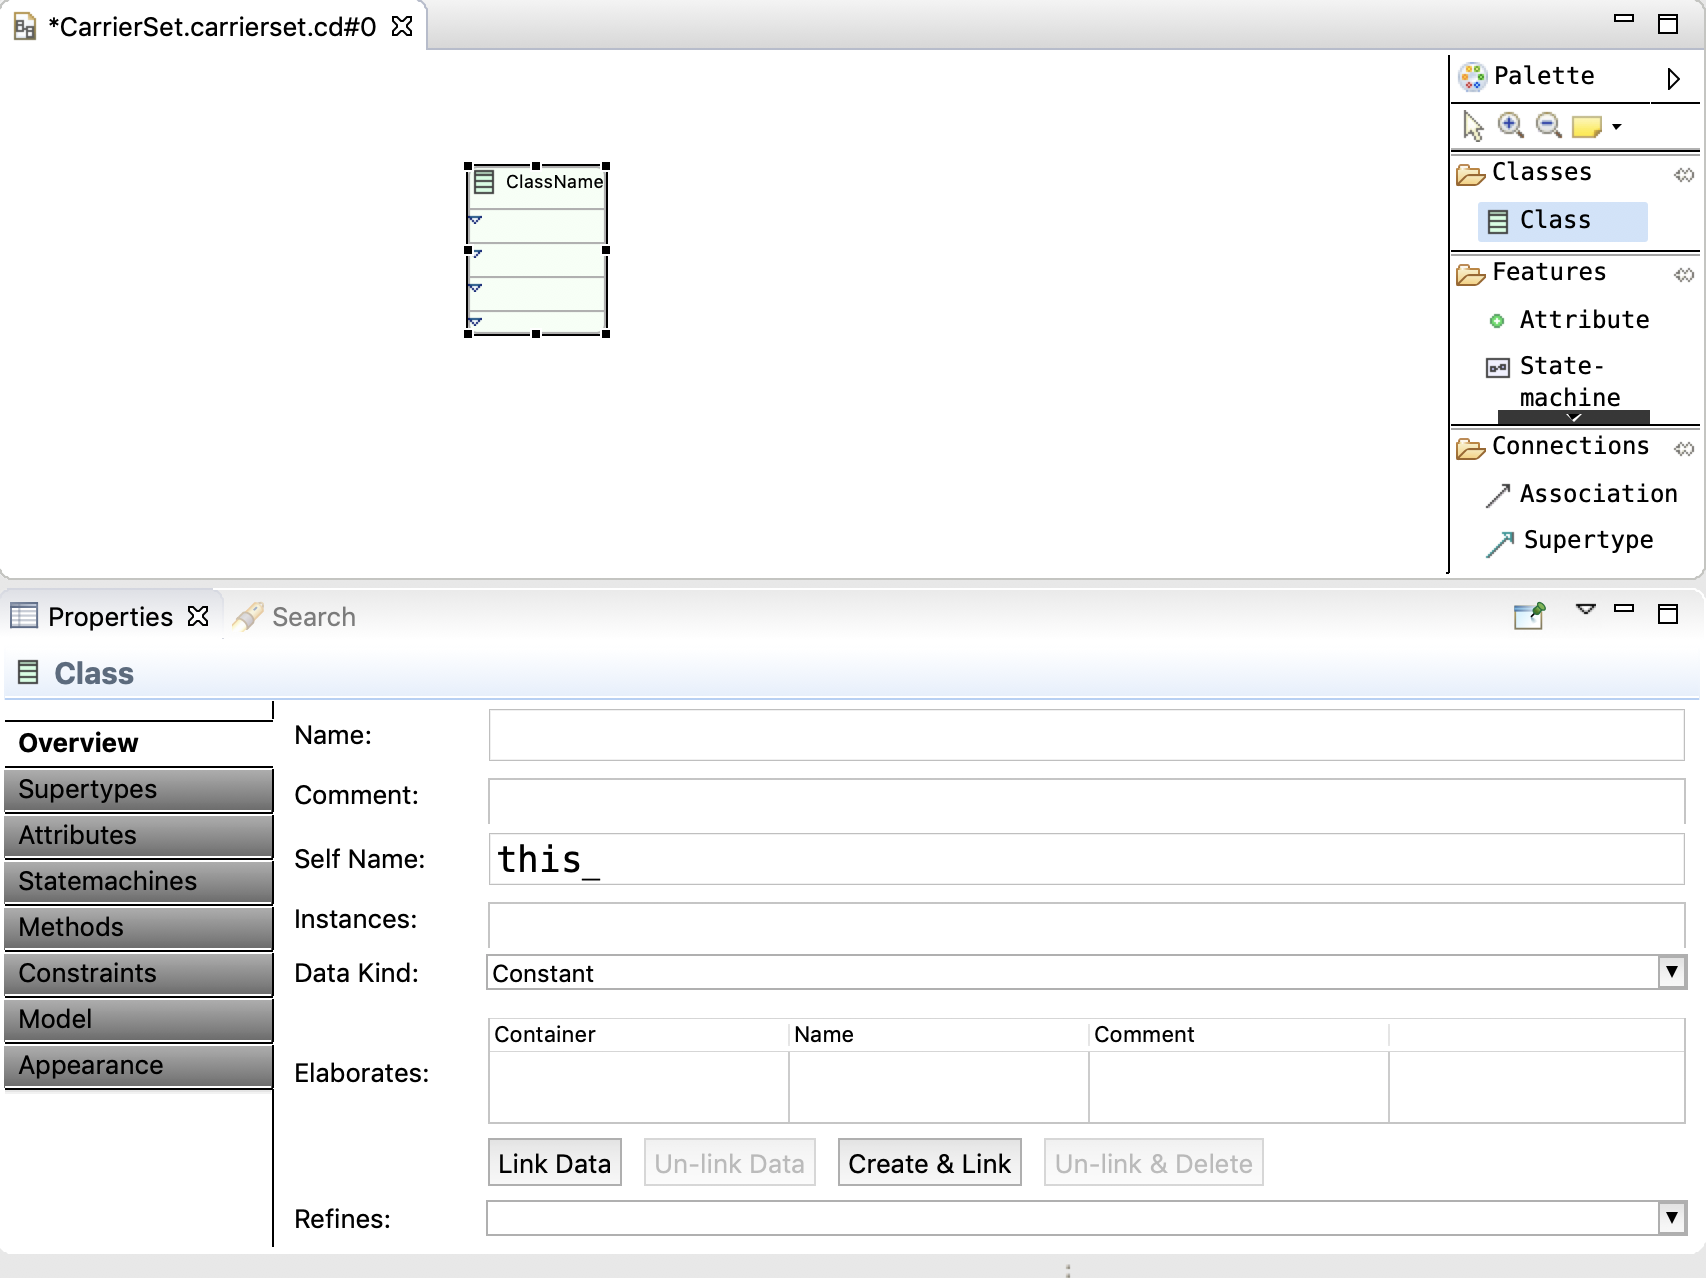
\includegraphics[width=1000]{figures/ClassCreation.png}
	\else
	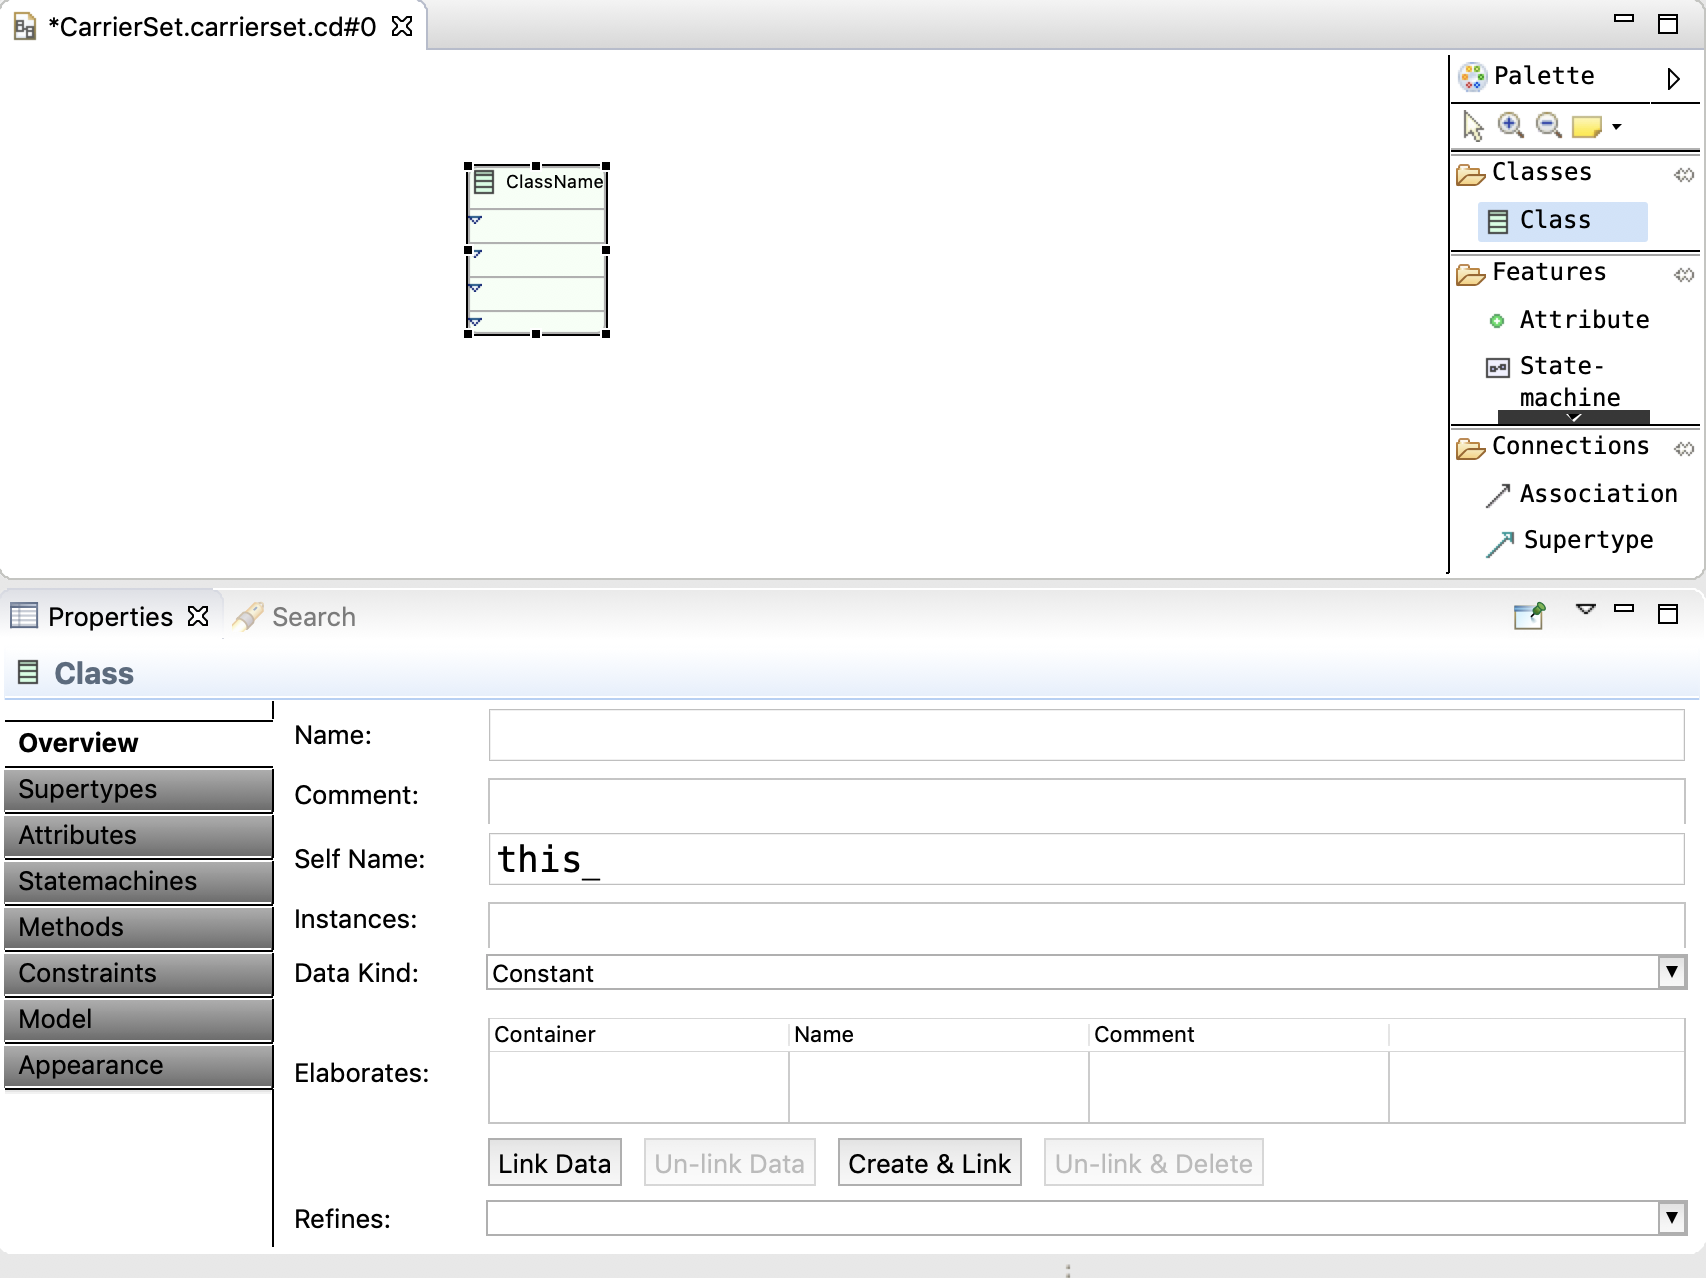
\includegraphics[width=1\textwidth]{figures/ClassCreation.png}
	\fi
	\caption{Class just created but not elaborated}
	\label{fig:ClassCreation}
\end{figure}

To set the elaboration of a class, use the buttons in the property view.
\begin{itemize}
	\item \command{Link Data} - adds a link to an existing data element in a machine or context
	\item \command{Un-link Data} - removes a link to a data element but leaves the data element
	\item \command{Create \& Link} - creates a new data element in a machine or context and links to it
	\item \command{Un-link \& Delete} - removes a link to a data element and also deletes the data element
\end{itemize}
\emph{Note: the \command{Create \& Link} and \command{Un-link \& Delete} buttons provide shortcuts to save you editing the machine or context. 
	The data elements are created/deleted from the machine/context as soon as you save the diagram. 
	These changes are NOT part of the translation.}

After setting the elaboration, the \code{Name} of the class, and its \code{Data Kind} property (Carrier Set, Constant or Variable) are updated automatically from the name and kind of the elaborated data. 
The rendering of the class changes automatically in the diagram to a yellow background to indicate that the elaborates property is set.
The icon in front of the class name changes to match that of the Event-B Explorer for the kind of data item that is elaborated (purple star = Carrier Set, yellow disc = Constant, green disc = Variable).
Fig.~\ref{fig:ClassElaboration} shows a class that \code{Elaborates} a carrier set.

\begin{figure}[!htbp]
	\centering
	\ifplastex
	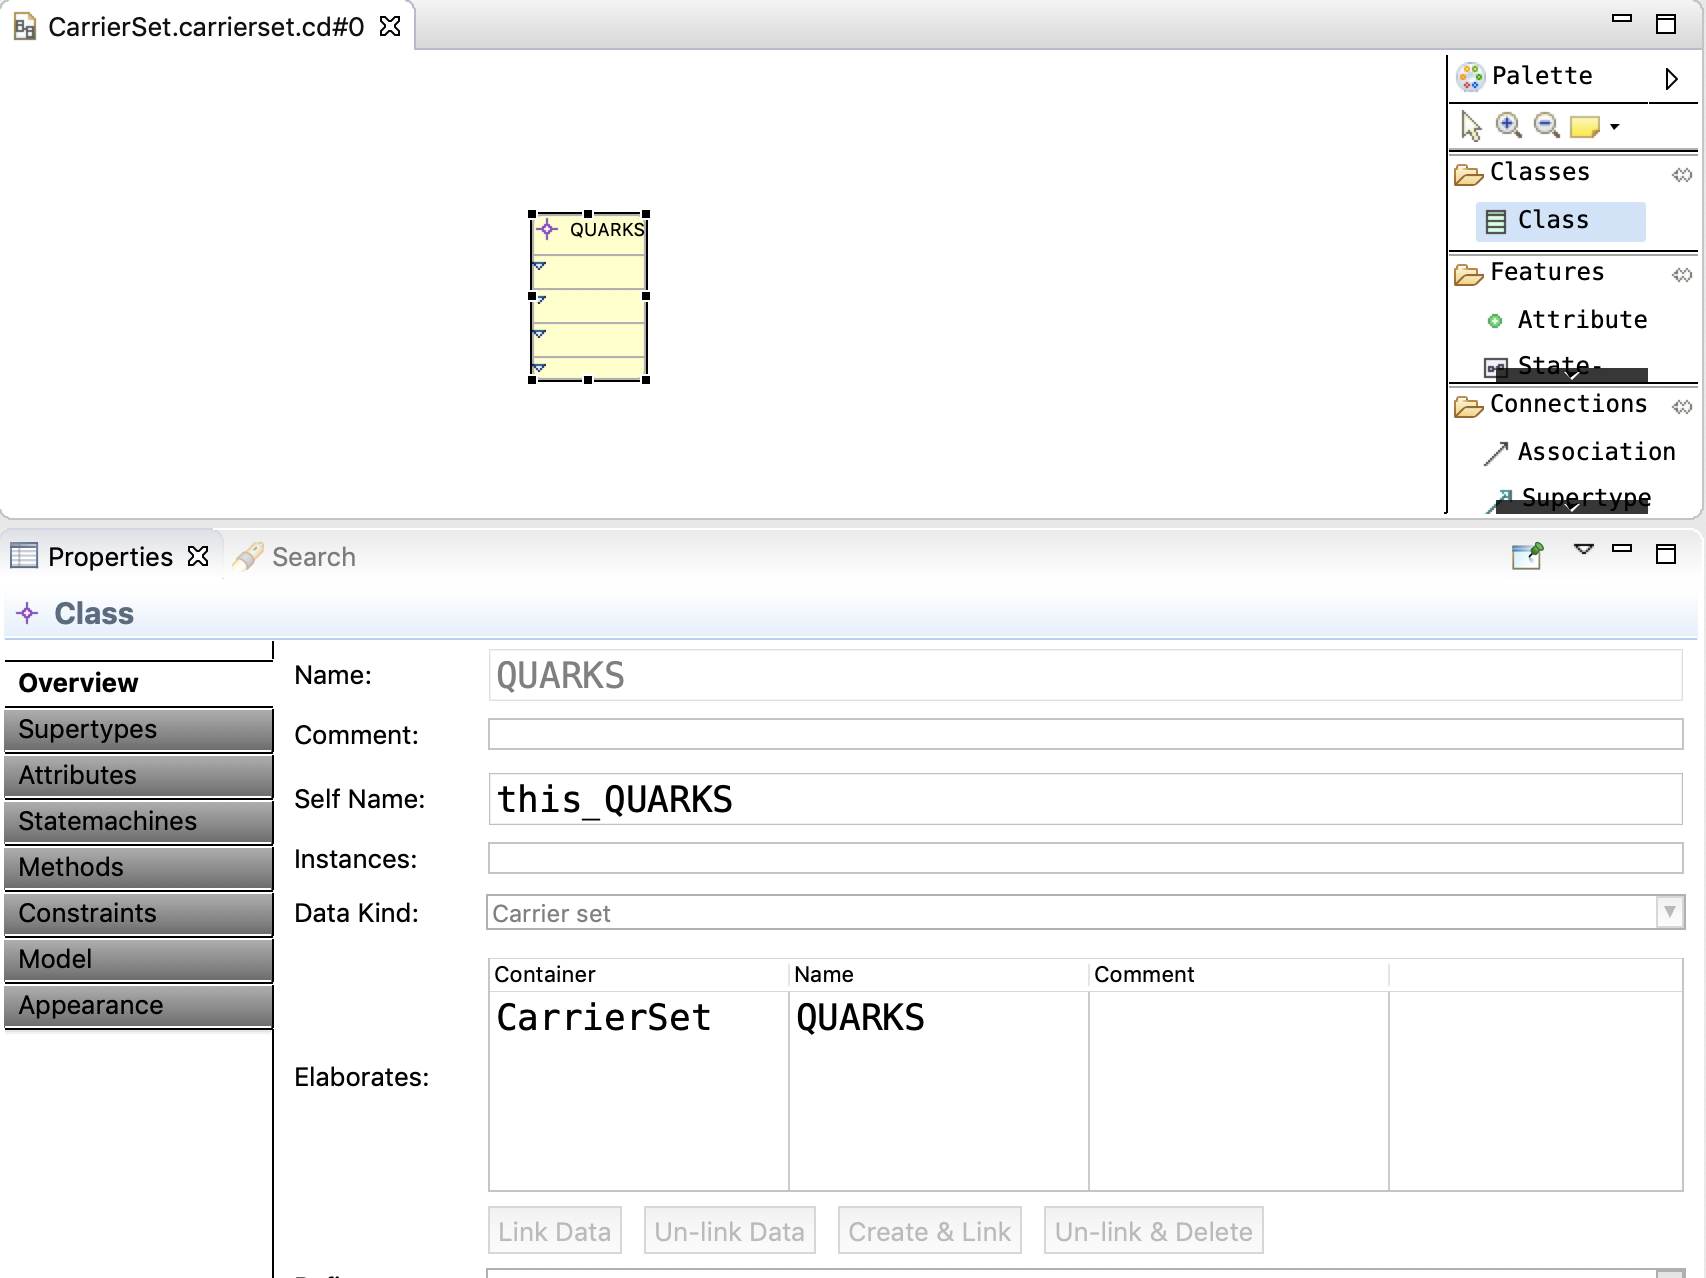
\includegraphics[width=1000]{figures/ClassElaboration.png}
	\else
	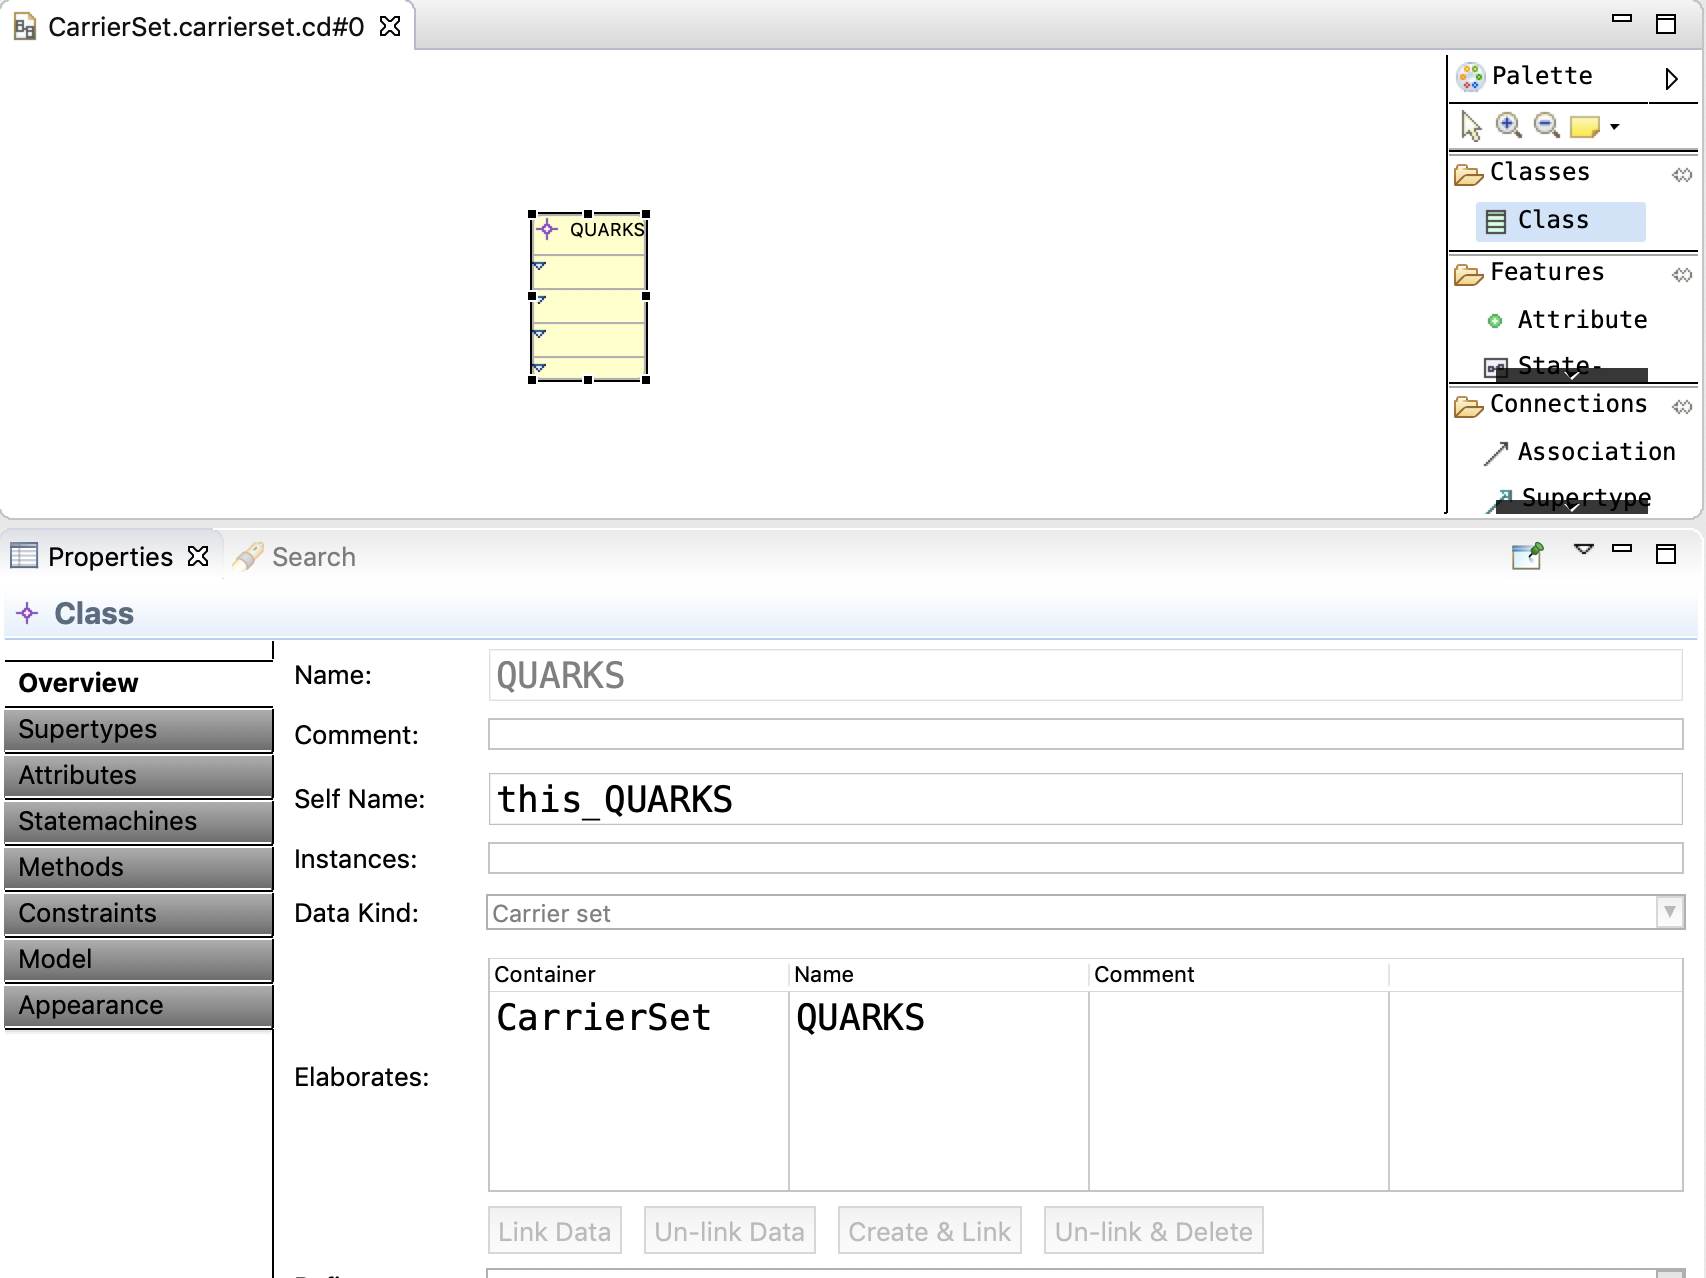
\includegraphics[width=1\textwidth]{figures/ClassElaboration.png}
	\fi
	\caption{Class that elaborates a Carrier Set}
	\label{fig:ClassElaboration}
\end{figure}

The \code{Self Name} property reserves an identifier for the contextual instance of the class (similar to this or self in O-O programming languages).
This identifier is used and/or recognised as the bound variable in quantifications over the class instances.
It is also used as the name of an automatically generated event parameter when the class has methods.
The default \code{Self Name}, shown in Fig.~\ref{fig:ClassElaboration}, is constructed by prepending \code{this\_} to the class name.


\begin{figure}[!htbp]
	\centering
	\ifplastex
	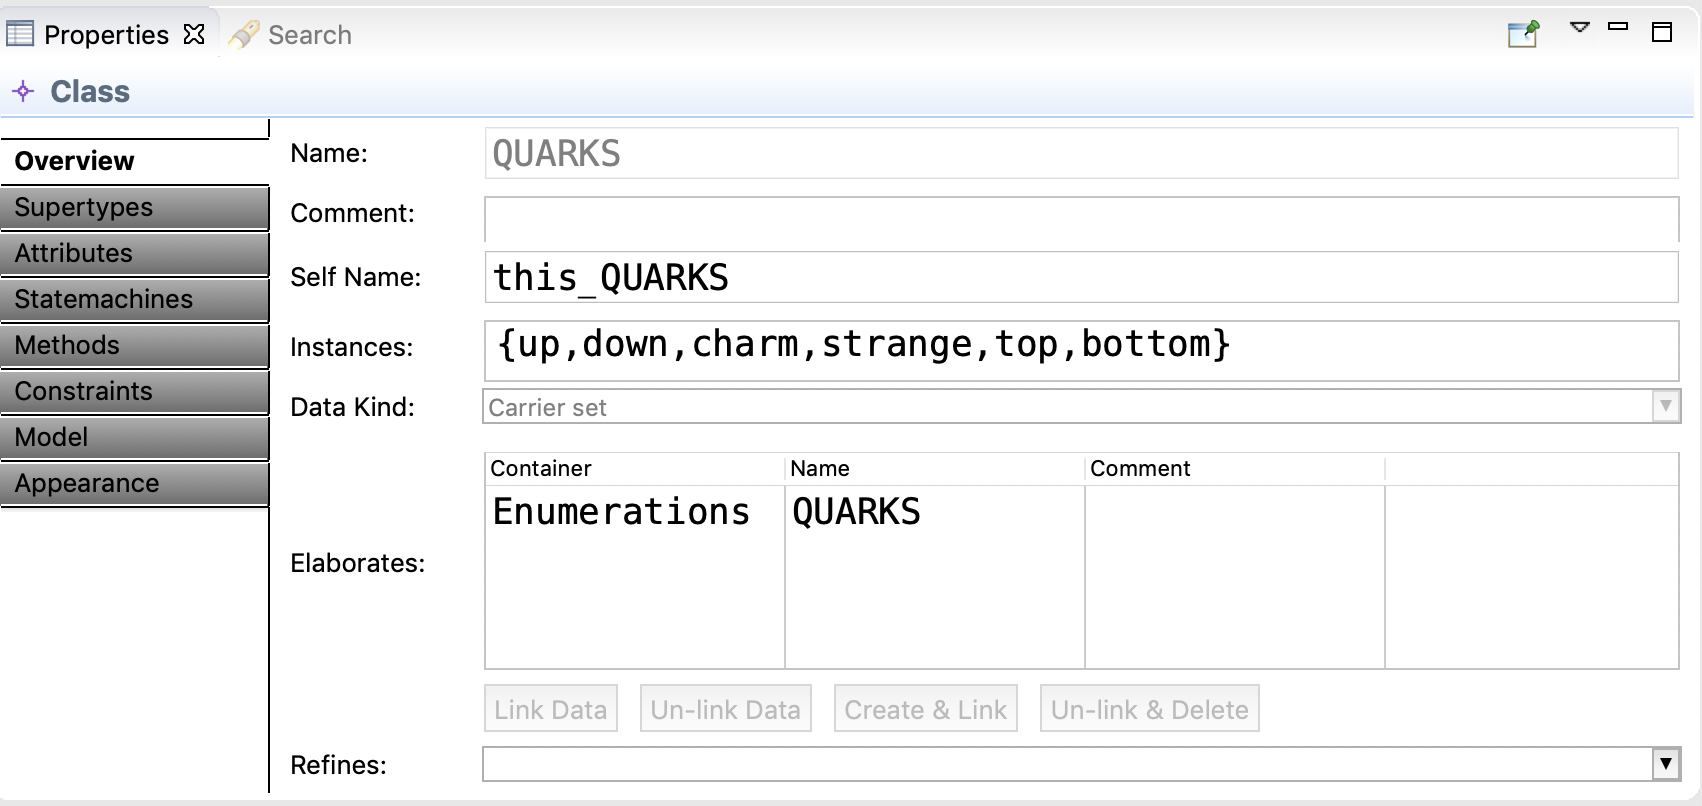
\includegraphics[width=1000]{figures/ClassEnumeration.png}
	\else
	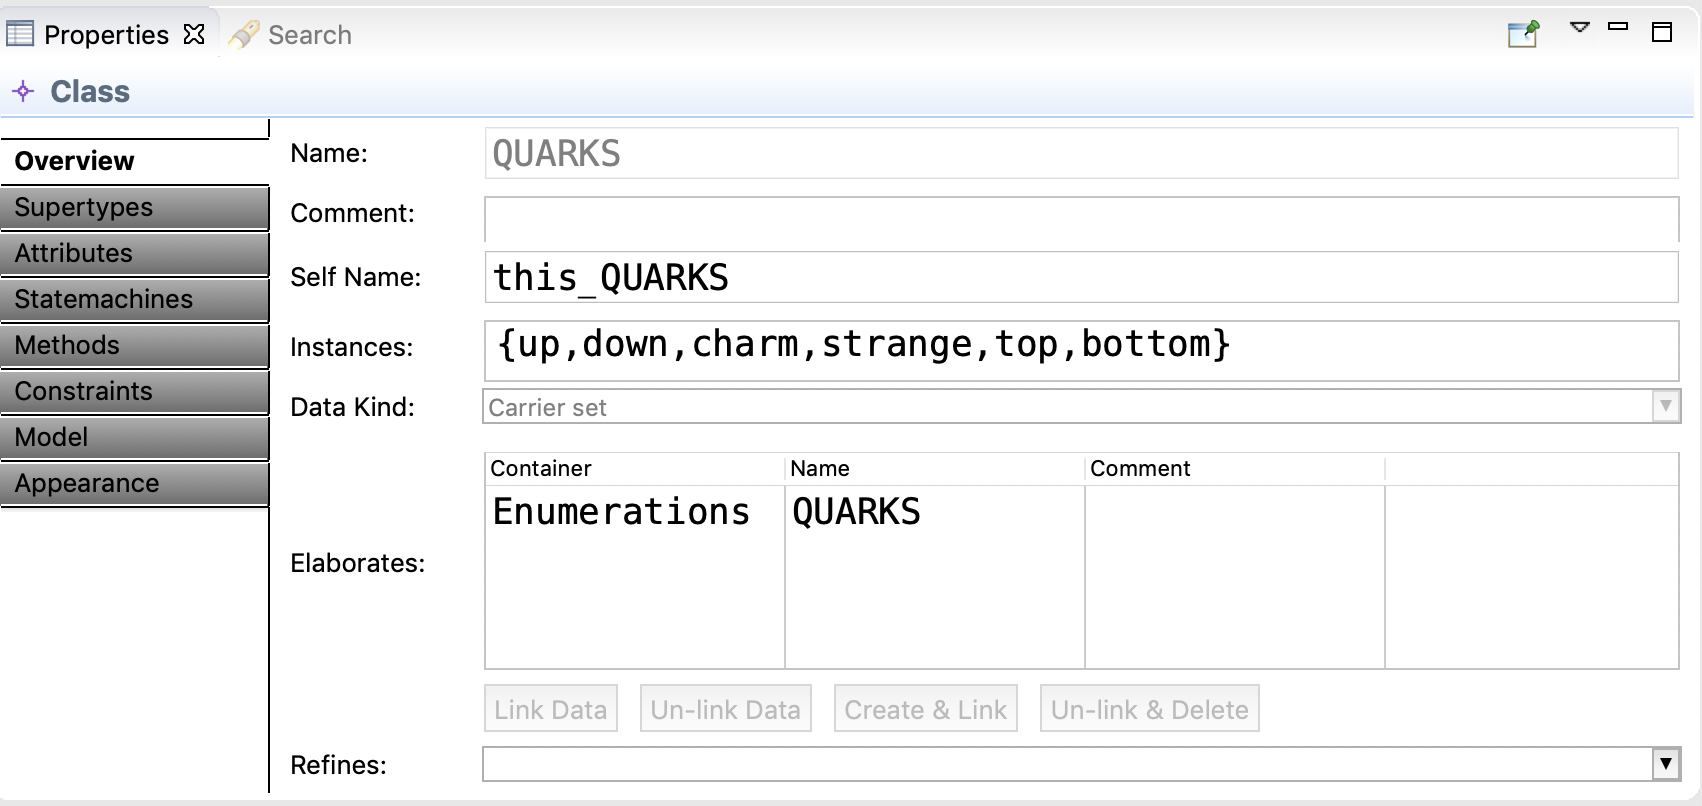
\includegraphics[width=1\textwidth]{figures/ClassEnumeration.png}
	\fi
	\caption{Class with instances that for an enumeration}
	\label{fig:ClassEnumeration}
\end{figure}


The \code{Instances} property can be used to specify the instances of the class.
For example, Fig.~\ref{fig:ClassEnumeration} shows the class instances specified as a set of labelled items.
The set brackets are recognised by the translation which generates a data element for each label and an axiom to ensure their uniqueness and coverage of the class.
The generated Event-B is:

\CONTEXT{Enumerations}{}{}
\SETS{
	\Set{QUARKS}{}
}
\CONSTANTS{
	\Constant{up}{instance of class QUARKS}
	\Constant{down}{instance of class QUARKS}
	\Constant{charm}{instance of class QUARKS}
	\Constant{strange}{instance of class QUARKS}
	\Constant{top}{instance of class QUARKS}
	\Constant{bottom}{instance of class QUARKS}
}
\AXIOMS{
	\Axiom{instancesOf\_QUARKS}{false}{$partition(QUARKS, \{up\},\{down\},\{charm\},\{strange\},\{top\},\{bottom\})$}{}
}
\END

The \code{refines} property allows you to select a class of a refined class diagram (i.e., in a machine refined by this diagram's machine).
Refinement of class diagrams will be explained in a later section.

 
